% "Isto vai ser um relatório" - Adriano Vinhas

\documentclass{article}
\usepackage[utf8]{inputenc}
\usepackage{graphicx}

\usepackage{color}

\newenvironment{text-blue}{\color{blue}}{}
\newenvironment{text-red}{\color{red}}{}

\begin{document}

\title{Máquina de calcular \\ Trabalho prático nº1, Computação Adaptativa}
\author{Adriano Vinhas (2009106560, avinhas@student.dei.uc.pt)\\
		José Ribeiro (2008112181, jbaia@student.dei.uc.pt}
\maketitle
\clearpage

% Introdução
\section{Introdução}

Este trabalho, no âmbito da disciplina de Computação Adaptativa, tem como objectivo construir uma rede neuronal capaz de reconhecer digítos (0-9) e operações aritméticas (+,-,=) de modo a ser capaz de servir como uma máquina de calcular.

Este objectivo foi atingido seguindo duas abordagens:
\begin{itemize}
\item Perceptrão
\item Memória Associativa Linear
\end{itemize}

A primeira abordagem é usada para resolver problemas linearmente separáveis e usa funções de activação saturadas. Esta abordagem procura estabelecer uma fronteira de decisão com base nos exemplos que existem para treino. Se existir uma solução possível, o procedimento de treino vai convergir. Para este trabalho, a função de activação usada no perceptrão é a \texttt{hardlim()}.

A segunda abordagem procura, através de dados de treino que permitam cobrir o maior espaço de procura possível (exemplos que sejam aceitáveis e ao mesmo tempo diferenciáveis entre si), treinar a rede de forma a ser tolerante ao ruído. Desta forma, se na altura de testar a rede surgirem exemplos semelhantes aos protótipos usados no treino, a saída deverá ser semelhante em relação a algum destes protótipos. Deste modo a rede é capaz de recordar os exemplos que foram usados para efectuar o seu treino. Em relação à função de activação, como o próprio nome indica, esta abordagem usa funções de activação lineares.

A parte que foi mais focada na realização deste trabalho foi a construção do dataset, de modo a explorar as situações acima enunciadas. Sumariamente, a construção do dataset foi feita tendo em mente o objectivo de ter diferentes possibilidades de dígitos que fizessem das redes tolerantes a ruído, sem que os erros introduzidos não fossem demasiado grandes e pudessem inviabilizar o bom desempenho destas.

% Treino da rede: Como foi feito o treino para cada um dos casos? Como foi feito o split de dados de validação e de treino?
% Que preocupações foram tidas em conta na hora de conceber o dataset
\clearpage
\section{A rede neuronal}
Nesta secção estão descritas a arquitectura da rede, já definida pelo professor no enunciado do trabalho, e as preocupações que se tiveram em conta na hora de treinar a rede.

\subsection{Arquitectura}
A arquitectura da rede neuronal usada para o trabalho prático caracteriza-se por 25 entradas, cada uma delas representando uma entrada binária da grelha usada para o preenchimento dos dígitos usando a função \texttt{mpaper()}, e 13 saídas, representando cada uma destas o digíto a ser escolhido.

As figuras~\ref{nn_architecture_perception} e~\ref{nn_architecture_lam} sumariam a arquitectura usada para a abordagem do perceptrão e da memória associativa linear, respectivamente.

\begin{figure}[!h]
  \centering
  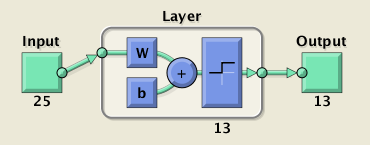
\includegraphics[width=3in]{figures/nn_architecture_perception}
  \caption{Arquitectura da rede neuronal usada no perceptrão para o trabalho prático 1}
  \label{nn_architecture_perception}
  
  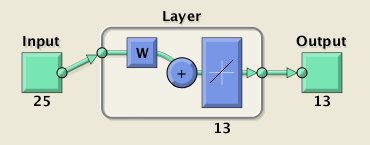
\includegraphics[width=3in]{figures/nn_architecture_lam}
  \caption{Arquitectura da rede neuronal usada na memória associativa linear para o trabalho prático 1}
  \label{nn_architecture_lam}
\end{figure}


\subsection{Treino da rede}
O dataset usado para este trabalho é composto por um total de 130 exemplos (10 exemplos para cada um dos 13 dígitos). Deste conjunto, 70\% dos exemplos (de cada dígito) foram usados para treinar a rede, e os restantes 30\% para validação desta e análise de resultados.

De referir que cada um dos conjuntos referidos anteriormente é seleccionado ao acaso, pelo que por cada vez que se corre o processo de constituição dos conjuntos de treino e validação, estes vão ter dígitos diferentes em cada conjunto, tendo como consequência pesos de diferentes valores e redes neuronais de diferentes performances. Para os resultados finais, seleccionou-se a matriz \texttt{W}, para cada uma das abordagens, que maximizava a performance destas.

Para todos os dígitos, procurou-se desenhar pelo menos um \textbf{dígito perfeito}. Os restantes exemplos foram construídos em função do dígito perfeito, introduzindo-se apenas pequenos erros ao modificar uma ou duas entradas ao dígito e criar os vários \textbf{dígitos imperfeitos}.

A figura~\ref{nn_dataset} representa o dataset utilizado para este trabalho.

\begin{figure}[!h]
  \centering
  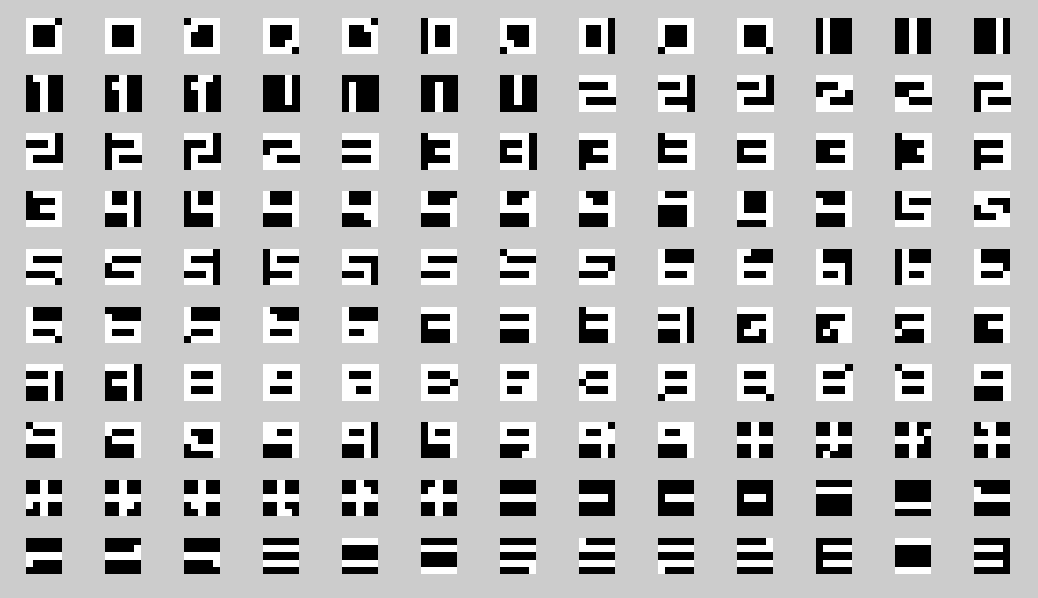
\includegraphics[width=5in]{figures/nn_dataset}
  \caption{Dataset do trabalho prático 1}
  \label{nn_dataset}
\end{figure}


% Gráficos com os resultados. Análise e interpretação.
\section{Resultados}
\begin{text-red} TODO!\end{text-red}
Nesta secção é feita uma análise de performance às duas abordagens usadas. Para este fim, 30 repetições foram levadas a cabo, cada uma destas com uma matriz de pesos diferentes para cada abordagem. Os resultados da figura~\ref{nn_long_run_performance} evidenciam a performance média para cada abordagem, usando 30 repetições.

\begin{figure}[!h]
  \centering
  \includegraphics[width=5in]{figures/nn_long_run_performance}
  \caption{Performance média das duas abordagens}
  \label{nn_long_run_performance}
\end{figure}




\end{document}
